\documentclass[11pt,xcolor={svgnames},aspectratio=169,usepdftitle=false]{beamer}

% Add space in lists
\let\toneitemize\itemize
\let\ttwoitemize\enditemize
\renewenvironment{itemize}{\toneitemize\addtolength{\itemsep}{0.7\baselineskip}}{\ttwoitemize}

\let\toneenumer\enumerate
\let\ttwoenumer\endenumerate
\renewenvironment{enumerate}{\toneenumer\addtolength{\itemsep}{0.7\baselineskip}}{\ttwoenumer}

% Alert color
\setbeamercolor{alerted text}{fg=DarkOrange}

% Itemize w bullets
\setbeamertemplate{itemize items}{$\circ$}

% Font size of title
\setbeamerfont{title}{size=\huge}

% Transition section slides
\setbeamertemplate{section page}
{
    \begin{centering}
    \begin{beamercolorbox}[sep=12pt,center]{part title}
        \setbeamerfont{section title}{size=\huge}
        \usebeamerfont{section title}\insertsection\par
    \end{beamercolorbox}
    \end{centering}
}

%===========================================================
% Color specifications
%===========================================================
\definecolor{GreyishBlue}{HTML}{087E8B} 	% Headings color
\definecolor{CitationsBlue}{HTML}{2B6684} 	% Color for citations
\definecolor{LinksPink}{HTML}{ff0054}       % Color for links

% Template for syntax highlighting
\definecolor{BeigeBackground}{HTML}{fdf6e3}
\definecolor{BlueKeyWord}{HTML}{268bd2}

\setbeamercolor{palette primary}{bg=GreyishBlue,fg=white}
\setbeamercolor{palette secondary}{bg=GreyishBlue,fg=white}
\setbeamercolor{palette tertiary}{bg=GreyishBlue,fg=white}
\setbeamercolor{palette quaternary}{bg=GreyishBlue,fg=white}
\setbeamercolor{structure}{fg=GreyishBlue} % itemize, enumerate, etc
\setbeamercolor{section in toc}{fg=GreyishBlue} % TOC sections
\setbeamercolor{background canvas}{bg=white}
\setbeamercolor{button}{bg=white, fg=GreyishBlue}

%===========================================================
% Numeration in environments
%===========================================================
\setbeamertemplate{theorems}[numbered]
\setbeamertemplate{definitions}[numbered]
\setbeamertemplate{navigation symbols}{}
\setbeamertemplate{caption}[numbered]

\usepackage{appendixnumberbeamer}

%===========================================================
% Language and font settings
%===========================================================
\usepackage[english,activeacute]{babel} % Language
\usefonttheme{professionalfonts}		% Avoid overwriting fonts

\usepackage[sfdefault,light]{FiraSans}
\usepackage[utf8]{inputenc}				% Special symbols
\usepackage[T1]{fontenc}				% T1 Encoding of font

%===========================================================
% Math font settings
%===========================================================
\usepackage{mathpazo}					% Math font
\usepackage{amsmath,amsfonts,amssymb}	% Math symbols
\usepackage{dsfont}						% Math symbols like R for reals...

%===========================================================
% References' colors and PDF properties
%===========================================================
\usepackage{hyperref}
\hypersetup
{
    pdfauthor={Rafael Serrano Quintero},
    pdfsubject={Introduction to Matlab},
    colorlinks = {true},
    linkcolor = {GreyishBlue},
    citecolor = {LinksPink},
    urlcolor = {LinksPink},
    filecolor = {LinksPink}
}
%===========================================================
% Additional packages
%===========================================================
\usepackage{graphicx}
\usepackage{tikz}

\usepackage{longtable}
\usepackage{appendix}
\usepackage{marvosym}
\usepackage{enumerate} %For enumerating with letters with option [a)]
\usepackage{epstopdf}
\usepackage[round]{natbib}
% Change manually the color of the parenthesis
\bibpunct{\textcolor{CitationsBlue}{(}}{\textcolor{CitationsBlue}{)}}{,}{a}{}{;}

\usepackage[flushleft]{threeparttable}
\usepackage{booktabs}
\usepackage[super]{nth}
\usepackage{float}
\usepackage{caption}
\usepackage{subcaption}
\usepackage{multicol}

%========================================================================================
% Syntax highlighting for Matlab
%========================================================================================
\usepackage{fancyvrb}  %To reduce font size in verbatim environment
\usepackage{listings}


\lstloadlanguages{Matlab}%
\lstset{
    language=Matlab,
    basicstyle=\footnotesize\ttfamily,
    backgroundcolor=\color{BeigeBackground}, 
    breaklines=true,                 
    captionpos=b,                    
    commentstyle=\color{gray},   
    frame=none,
    keywordstyle=[1]\color{BlueKeyWord}\bfseries, % MATLAB functions bold and blue
    keywordstyle=[2]\color{Purple},  % MATLAB function arguments purple
    keywordstyle=[3]\color{Purple}\underbar,  % User functions underlined and blue      
    stringstyle=\color{Purple},   
    morekeywords={xlim,ylim,var,alpha,factorial,poissrnd,normpdf,normcdf,ones},
    %Put MATLAB function parameters here
    morekeywords=[2]{all, on, off, interp},
    morecomment=[s]{\%\{}{\%\}},
    numbers=left,                    
    numbersep=3pt,                   
    numberstyle=\tiny\color{black},
    rulecolor=\color{black},        
    showspaces=false,               
    showstringspaces=false,          
    showtabs=false,                  
    stepnumber=1,                    
    tabsize=2         
}

\newtheorem{exercise}{Exercise}
%===========================================================
% DOCUMENT
%===========================================================
\title{Introduction to Matlab}
\subtitle{Lesson 02 --- Importing, manipulating, and fitting Data}

\author{Rafael Serrano-Quintero}

\institute{Department of Economics \\ University of Barcelona}
\date{}

\AtBeginSection[]{\frame{\sectionpage}}
\AtBeginSubsection[]{\frame{\subsectionpage}}

\defbeamertemplate{section page}{mine}[1][]{%
  \begin{centering}
    {\usebeamerfont{section name}\usebeamercolor[fg]{section name}#1}
    \vskip1em\par
    \begin{beamercolorbox}[sep=12pt,center]{part title}
      \usebeamerfont{section title}\insertsection\par
    \end{beamercolorbox}
  \end{centering}
}

\defbeamertemplate{subsection page}{mine_sub}[1][]{%
  \begin{centering}
    {\usebeamerfont{subsection name}\usebeamercolor[fg]{subsection name}#1}
    \vskip1em\par
    \begin{beamercolorbox}[sep=12pt,center]{part title}
      \usebeamerfont{subsection title}\insertsubsection\par
    \end{beamercolorbox}
  \end{centering}
}

\setbeamertemplate{section page}[mine]
\setbeamertemplate{subsection page}[mine_sub]

\begin{document}

\VerbatimFootnotes

\maketitle

\section{Importing and Manipulating Data}

\begin{frame}[fragile]
    \frametitle{Importing and Manipulating Data}
\begin{itemize}
    \item Download the data from the World Bank in CSV.
    \begin{itemize}
        \item \href{https://data.worldbank.org/indicator/NY.GDP.PCAP.KD}{GDP per capita (constant 2010 US\$)}
        \item \href{https://data.worldbank.org/indicator/SP.URB.TOTL.IN.ZS}{Urban population as a \% of total population}
    \end{itemize}
    \item Rename to \verb;urban_pop.csv; and \verb;real_gdp_percapita.csv;
    \item Forget by now about the metadata files.
    \item Download in a subdirectory in the working directory as \verb;working_directory/data/;
\end{itemize}
\end{frame}

\begin{frame}[fragile]
  \frametitle{Importing and Manipulating Data}
\begin{itemize}
  \item Since the data files have \textit{headers} or column names, we explicitly tell the command that.
  \item Let's import the data as a table using \verb;readtable();
\end{itemize}
\begin{lstlisting}
close all
clear
clc

% Importing data from CSV file
gdp = readtable('./data/real_gdp_percapita.csv','ReadVariableNames',true);
pop = readtable('./data/urban_pop.csv','ReadVariableNames',true);  
\end{lstlisting}
\end{frame}

\begin{frame}[fragile]
  \frametitle{Importing and Manipulating Data}
\begin{itemize}
  \item \href{https://www.mathworks.com/help/matlab/tables.html}{Tables in Matlab} are a data type created to store data that is column oriented.
  \item They are not like arrays, we need to extract the numeric columns.
  \item Let's find out if country codes are the same for both variables.
  \item To make manipulation easier, transform to a \href{https://www.mathworks.com/help/matlab/ref/cell.html}{cell array}.
\end{itemize}
\begin{lstlisting}
% Extract CountryCode for both files
ccode_gdp = table2cell(gdp(:,2));
ccode_pop = table2cell(pop(:,2));
\end{lstlisting}
\end{frame}

\begin{frame}[fragile]
  \frametitle{Importing and Manipulating Data}
  To check if country codes coincide:
  \begin{enumerate}
    \item Compare one by one.
    \item Check if all elements are \verb;true;
  \end{enumerate}
\begin{lstlisting}
% Compare strings one by one
compare_ccode = strcmp(ccode_gdp,ccode_pop);
all_true = all(compare_ccode);
disp(all_true)
\end{lstlisting}
Since they are, we can safely merge the two variables.
\end{frame}

\begin{frame}[fragile]
  \frametitle{Importing and Manipulating Data}
\begin{itemize}
  \item Extract the numeric values of GDP and urban population.
  \item We use \verb;table2array(); to convert into a matrix.
  \item We transpose so that each row is a year and each column a country.
\end{itemize}
\begin{lstlisting}
% Extract GDP per capita and urban population as a matrices
gdp_pc = table2array(gdp(:,5:end))';
pop_ub = table2array(pop(:,5:end))';
\end{lstlisting}
\end{frame}

\begin{frame}[fragile]
  \frametitle{Importing and Manipulating Data}
\begin{itemize}
  \item Explore the rough relationship between $\log(GDP)$ and urban population.
  \item To do a pooled scatter plot use the \verb;(:); operator. This converts a matrix into a vector.
\end{itemize}
\begin{lstlisting}
% Explore the relationship between GDPpc and Urban population
figure
scatter(log(gdp_pc(:)),pop_ub(:),...
      'filled','MarkerFaceAlpha',0.25)
hold on
lsline % add a least squares line

% Rough correlation
disp(corrcoef(log(gdp_pc(:)),pop_ub(:),'Rows','complete'))
\end{lstlisting}
\end{frame}

\begin{frame}[fragile]
  \frametitle{Importing and Manipulating Data}
\begin{itemize}
  \item The correlation for all countries is $0.8290$. Let's explore the correlation for each country individually.
\end{itemize}
\begin{lstlisting}
% Correlation by country
[T, N] = size(gdp_pc); % Time periods (T) and number of countries (N)

corr_coefs = zeros(N,1);
for n = 1:N
    tmp = corrcoef(log(gdp_pc(:,n)),pop_ub(:,n),'Rows','Complete');
    corr_coefs(n,1) = tmp(1,2);
end

mean(corr_coefs,'omitnan')
\end{lstlisting}
\begin{itemize}
  \item The average is $0.54$ and the standard deviation $0.60$.
\end{itemize}
\end{frame}

\begin{frame}[fragile]
  \frametitle{Importing and Manipulating Data}
\begin{exercise}
Plot the evolution over time for a particular country. Plot the two series in the same graph with two different $y-$axes. Also, make sure you include the years in the $x-$axis.
\end{exercise}
\end{frame}

\begin{frame}[fragile]
  \frametitle{Importing and Manipulating Data}
How has it been for India?

\begin{minipage}{0.45\textwidth}
\begin{lstlisting}
% Plot the evolution for India
years = 1960:1960+T-1;
india = strcmp(ccode_gdp,'IND');
gdp_india = gdp_pc(:,india);
urb_india = pop_ub(:,india);
  
figure
plot(years,gdp_india,'-o')
hold on
yyaxis right
plot(years,urb_india,'-s')
\end{lstlisting}
\end{minipage}
\begin{minipage}{0.45\textwidth}
\begin{figure}
  \centering
  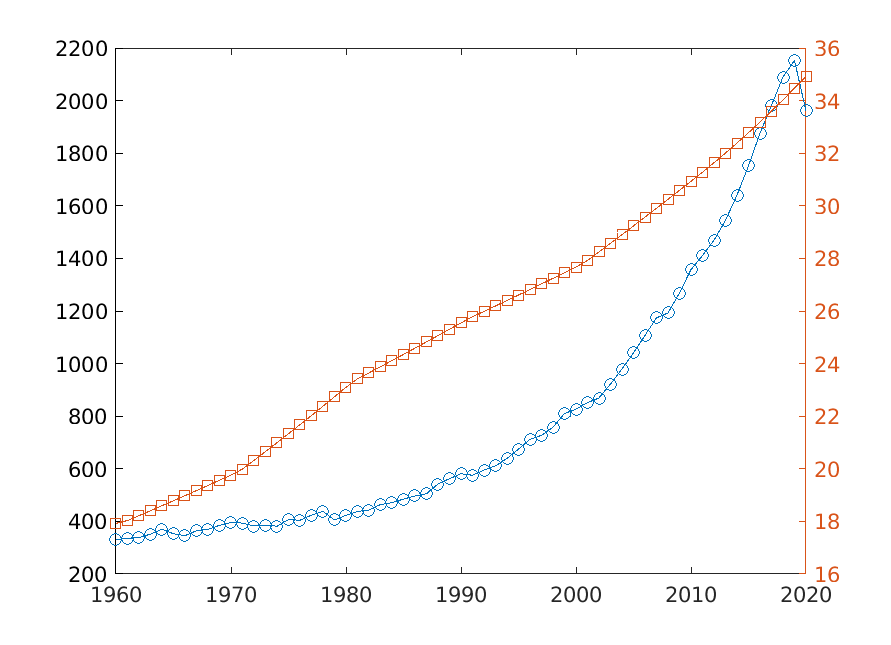
\includegraphics[width = \textwidth]{../figures/india_gdp_urb.png}
  \caption{Real GDPpc and Urban Pop}
  \label{fig:india_evolution}
\end{figure}
\end{minipage}
\end{frame}

\section{Fitting Data}

\subsection{Linear Regression}

\begin{frame}[fragile]
  \frametitle{Linear Regression}
\begin{itemize}
  \item Let's estimate a linear regression for the relationship between GDP per capita and urban population with a time trend.
  \[
  \log(GDPpc_{t,i}) = \beta_0 + \beta_1 urban_{t,i} + \beta_2 time_t + \varepsilon_{t,i}
  \]
  \item The OLS estimator is $\hat{\beta} = (X'X)^{-1}X'y$ where
  \[
  X = \begin{pmatrix}
    1 & urban_{1960,1} & 1960 \\
    \vdots & \vdots & \vdots \\
    1 & urban_{2020,N} & 2020 
  \end{pmatrix}  \ 
  y = \begin{pmatrix}
    \log(GDPpc_{1960,1}) \\
    \vdots \\
    \log(GDPpc_{2020,N})
  \end{pmatrix}
  \]
\end{itemize}
\end{frame}

\begin{frame}[fragile]
  \frametitle{Linear Regression}
Necessary steps:
\begin{enumerate}
  \item Reshape matrices into vectors of size $T\times N$ and create $time_t$.
\end{enumerate}
\begin{lstlisting}
% Reshape GDPpc matrix into a vector
y = reshape(gdp_pc,[T*N,1]);
y = log(y);     % Recall our dependent variable is in logs!

% Reshape pop_ub in the same way
urb_vect = reshape(pop_ub,[T*N,1]);

% Create the time trend
years_mat = repmat(years,N,1);
years_mat = years_mat';
years_vec = reshape(years_mat,[T*N,1]);
\end{lstlisting}
\end{frame}

\begin{frame}[fragile]
  \frametitle{Linear Regression}
Necessary steps:
\begin{enumerate}
  \setcounter{enumi}{1}
  \item Remove missing values from all variables.
\end{enumerate}
\begin{lstlisting}
% Remove missing values from both variables
miss_y = isnan(y);
miss_u = isnan(urb_vect);
tot_miss = logical(miss_y + miss_u);

y_clean = y(~tot_miss);
u_clean = urb_vect(~tot_miss);
years_vec = years_vec(~tot_miss);
\end{lstlisting}
\end{frame}

\begin{frame}[fragile]
  \frametitle{Linear Regression}
Necessary steps:
\begin{enumerate}
  \setcounter{enumi}{2}
  \item Construct $X$ and compute $\hat{\beta}$
\end{enumerate}
\begin{lstlisting}
% Create matrix X
X = [ones(size(u_clean)), u_clean, years_vec];

% Estimate bhat
bhat = ((X')*X)\((X')*y_clean);
\end{lstlisting}
\[
\hat{\beta} = \begin{pmatrix}
11.0201 \\
\phantom{-}0.0509  \\
-0.0027 \\
\end{pmatrix}
\]
So, $\Delta urban = 1$ percentage point is associated with $\Delta GDPpc =  5.09\%$. \alert{\textbf{NOT A CAUSAL RELATIONSHIP!!!}}
\end{frame}

\begin{frame}[fragile]
  \frametitle{Linear Regression --- Other Ways}
\begin{itemize}
  \item What if we want standard errors, p-values \ldots ?
  \item Fortunately, we do not need to compute them by hand.
  \item We are going to see \href{https://www.mathworks.com/help/stats/fitlm.html?s_tid=doc_ta}{\texttt{fitlm}} and \href{https://www.mathworks.com/help/stats/linearmodel.html}{\texttt{LinearModel}}.
  \item These are found within the \href{https://www.mathworks.com/help/stats/index.html?s_tid=CRUX_lftnav}{Statistics and Machine Learning Toolbox}.
  \item Alternatives:
  \begin{itemize}
    \item \href{https://www.mathworks.com/help/curvefit/fit.html?s_tid=doc_ta}{\texttt{fit}} from the \href{https://www.mathworks.com/help/curvefit/index.html?s_tid=CRUX_lftnav}{Curve Fitting Toolbox}
    \item \href{https://www.mathworks.com/help/stats/regress.html}{\texttt{regress}} from the \href{https://www.mathworks.com/help/stats/index.html?s_tid=CRUX_lftnav}{Statistics and Machine Learning Toolbox}
    \item \href{https://www.spatial-econometrics.com/}{Spatial Econometrics Toolbox} by James P. LeSage.
    \item Much more recommended for serious data work \href{https://www.r-project.org/}{R}, \href{https://www.stata.com/}{Stata}, \href{https://www.python.org/}{Python}
  \end{itemize}
\end{itemize}
\end{frame}

\begin{frame}[fragile]
  \frametitle{Linear Regression --- \texttt{fitlm} and \texttt{LinearModel}}
\begin{itemize}
  \item \texttt{fitlm} creates a \texttt{LinearModel} object, estimates the model, and produces results for that particular model object.
  \item \texttt{fitlm} accepts data in \verb;table; format or numeric array format. We will stick to numeric array.
  \item By default it includes a constant and deals with missing values.
\end{itemize}
\begin{lstlisting}
% Control variables
Xfitlm = [urb_vect, years_vec];

% Model object
linmodel = fitlm(Xfitlm,y);
disp(linmodel)
\end{lstlisting}
\end{frame}

\begin{frame}[fragile]
  \frametitle{Linear Regression --- \texttt{fitlm} and \texttt{LinearModel}}
  The default output of the \verb;fitlm; model includes
\begin{itemize}
  \item Coefficients, standard errors, $t-$statistics, $p-$values \ldots
  \item Reassuringly, we get the same coefficients as before.
\end{itemize}
\begin{lstlisting}[basicstyle=\tiny\ttfamily]
>> disp(linmodel)

Linear regression model:
    y ~ 1 + x1 + x2

Estimated Coefficients:
                    Estimate         SE         tStat       pValue  
                   __________    __________    _______    __________

    (Intercept)         11.02       0.92273     11.943    1.0777e-32
    x1               0.050911    0.00032252     157.86             0
    x2             -0.0026586     0.0004651    -5.7161    1.1155e-08


Number of observations: 12131, Error degrees of freedom: 12128
Root Mean Squared Error: 0.821
R-squared: 0.688,  Adjusted R-Squared: 0.688
F-statistic vs. constant model: 1.34e+04, p-value = 0
\end{lstlisting}
\end{frame}

\begin{frame}[fragile]
  \frametitle{Linear Regression --- \texttt{fitlm} and \texttt{LinearModel}}
We can perform some model diagnostics
\begin{itemize}
  \item \verb;plotResiduals(linmodel); to show a histogram of residuals.
  \item \verb;plotResiduals(linmodel,'fitted'); residuals vs fitted values.
  \item \verb;plotEffects(linmodel); to show size of coefficients.
\end{itemize}
We can access directly several derived objects
\begin{itemize}
  \item \verb;linmodel.LogLikelihood; the log-likelihood.
  \item \verb;linmodel.Residuals; the residuals of the fitted model.
  \item \verb;linmodel.Coefficients; the value of estimated coefficients.
\end{itemize}
\end{frame}

\subsection{Polynomial Fit and Polynomial Evaluation}

\begin{frame}
  \frametitle{Polynomial Fit}
\begin{theorem}[Weierstrass' Approximation Theorem]
Let $f(x)$ be a continuous real-valued function defined on $[a,b]$. Then, given $\varepsilon$ we can find a polynomial $p(x)$ such that
\[
\sup \lvert f(x) - p(x) \rvert < \varepsilon  
\]
\end{theorem}
\textit{Informally:} any continuous function on $[a,b]$ can be approximated well by a polynomial function.
\end{frame}

\begin{frame}
  \frametitle{Polynomial Fit}
\begin{itemize}
  \item Suppose, we have the following relationship between $y$ and $x$
  \[
  y = \sin(5\times x^2 + \pi)
  \]
  with $x\in\mathbb{R}$. Note that the function is continuous in $\mathbb{R}$.
  \item But we do not know the relationship. Let us approximate by an $n-$degree polynomial using Matlab.
  \item This is done with the commands \href{https://www.mathworks.com/help/matlab/ref/polyfit.html}{\texttt{polyfit}} and \href{https://www.mathworks.com/help/matlab/ref/polyval.html}{\texttt{polyval}} to fit and evaluate polynomials respectively. \footnotesize (How exactly are we fitting\ldots ?)
\end{itemize}
\end{frame}

\begin{frame}[fragile]
  \frametitle{Polynomial Fit}
  \begin{itemize}
    \item Let's fit the data using \nth{5}, \nth{6}, and \nth{7} degree polynomials.
    \item Evaluate them and plot them.
  \end{itemize}

\begin{minipage}{0.45\textwidth}
\begin{lstlisting}
% Simulate variables and their relationship
x = linspace(-1,1,1000);
y = sin(5.*x.^2 + pi);
  
% Fit 5,6,7th degree polynomials
p5 = polyfit(x,y,5);
p6 = polyfit(x,y,6);
p7 = polyfit(x,y,7);
\end{lstlisting}
\end{minipage}
\begin{minipage}{0.45\textwidth}
\begin{figure}
  \centering
    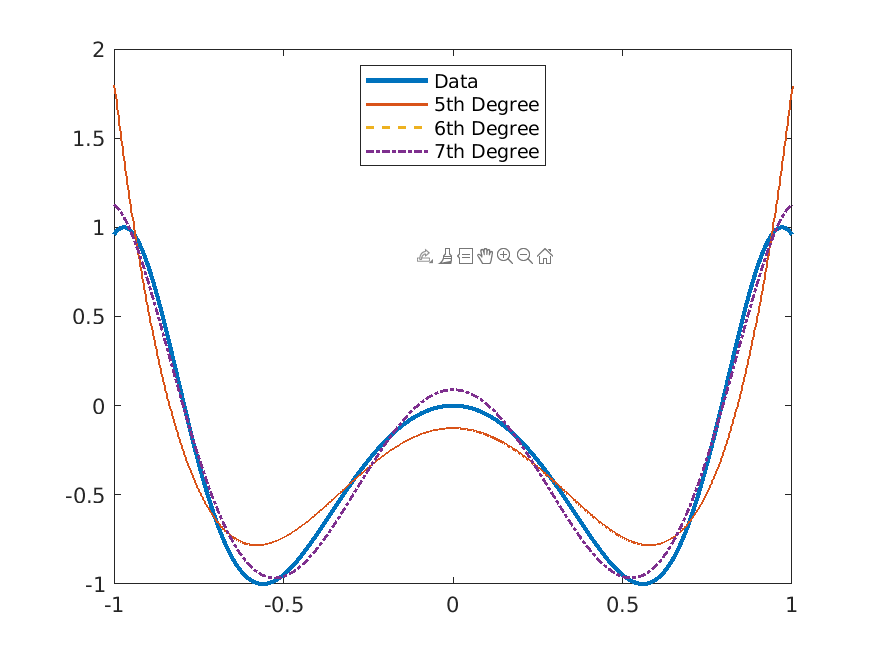
\includegraphics[width = \textwidth]{../figures/poly_fit.png}
\end{figure}
\end{minipage}
\end{frame}

\begin{frame}
    \frametitle{Polynomial Fit}
\begin{exercise}
Simulate a variable $x$ in the interval $[-4,4]$ with $1000$ points. Generate a variable $y = x^2 + \varepsilon$ where $\varepsilon$ is white noise with standard  deviation $1.5$. Fit a second degree polynomial and plot the simulated data and the fitted polynomial on the same plot.
\end{exercise}
\end{frame}

\begin{frame}[fragile]
  \frametitle{Polynomial Fit}
Fitting data with noise.
\begin{lstlisting}
X = linspace(-4,4,1000);
Y = X.^2 + 1.5.*randn(1,length(X));
p2 = polyfit(X,Y,2);

figure
scatter(X,Y)
hold on
plot(X,polyval(p2,X),'-','LineWidth',1.35)
title('Polynomial Fit')
\end{lstlisting}
\end{frame}

\subsection{Nonlinear Least Squares}

\begin{frame}[fragile]
  \frametitle{Nonlinear Least Squares}
\begin{itemize}
  \item Consider a set of data points $(x_1,y_1),\ldots,(x_N,y_N)$ and a function $y = f(x,\beta)$ depending on unknown parameters $\beta = (\beta_1,\ldots,\beta_m)$ where $N > m$.
  \item The Nonlinear Least Squares estimator is the set of coefficients $\beta$ such that
  \[
  \underset{\beta}{\min} \sum^N_{i=1} (y_i - f(x_i,\beta))^2
  \]
  \item \verb;polyfit; is exactly doing that but when $f(x,\beta)$ is a polynomial of degree $n$.
  \item We can extend that to \alert{\textbf{any}} nonlinear function easily.
\end{itemize}
\end{frame}

\begin{frame}[fragile]
  \frametitle{Nonlinear Least Squares --- Anonymous Functions}
  \begin{itemize}
    \item Before we dive into NLLS fitting, let's introduce \href{https://www.mathworks.com/help/matlab/matlab_prog/anonymous-functions.html}{anonymous functions}.
    \item We learned in previous lecture about user defined functions. Anonymous functions are functions \alert{\textit{not stored in an}\texttt{.m} \textit{file}}.
    \item These functions work within a script and they are stored in the workspace as \href{https://www.mathworks.com/help/matlab/ref/function_handle.html}{\texttt{function\_handle}} objects.
    \item To create an anonymous function that multiplies a number by two:
  \end{itemize}
\begin{lstlisting}
% Create the function
bytwo = @(x) 2*x;
% Call it
a = bytwo(10);
\end{lstlisting}
\end{frame}

\begin{frame}[fragile]
  \frametitle{Nonlinear Least Squares --- Functions}
\begin{itemize}
  \item To perform NLLS Matlab provides several alternatives
  \item We will focus on \href{https://www.mathworks.com/help/optim/ug/lsqcurvefit.html}{\texttt{lsqcurvefit}}. Other alternatives are
  \begin{itemize}
    \item \href{https://www.mathworks.com/help/optim/ug/lsqnonlin.html}{\texttt{lsqnonlin}}
    \item \href{https://www.mathworks.com/help/stats/nlinfit.html}{\texttt{nlinfit}}
    \item \href{https://www.mathworks.com/help/stats/fitnlm.html}{\texttt{fitnlm}} (very similar to \texttt{fitlm})
  \end{itemize}
  \item \texttt{lsqcurvefit} and \texttt{lsqnonlin} are \alert{\textbf{equivalent}} since they use the same algorithm.
  \item We will focus on \href{https://www.mathworks.com/help/optim/ug/lsqcurvefit.html}{\texttt{lsqcurvefit}} provides a convenient way of writing the problem and advances syntax for the lecture on optimization.
\end{itemize}
\end{frame}

\begin{frame}[fragile]
  \frametitle{Nonlinear Least Squares --- \texttt{lsqcurvefit}}
  \begin{itemize}
    \item Suppose we want to fit a data generating process of the type
    \[
    y = b_1 \exp(b_2 x) + \varepsilon \ \text{ where } \varepsilon \thicksim \mathcal{N}(0,0.15) \text{ and } x\in [0,5]
    \]
    \item Suppose we have $N$ pairs of observations $(x_i,y_i)$ and we want to find parameters $b_1$ and $b_2$ that best fit the data.
    \item Let's simulate the data first
  \end{itemize}
\begin{lstlisting}
%Simulate data
N = 500;
b1 = 2;
b2 = -1.5;
x = linspace(0,5,N);
y = b1*exp(b2*x)+0.15*randn(1,N);
\end{lstlisting}
\end{frame}

\begin{frame}[fragile]
  \frametitle{Nonlinear Least Squares --- \texttt{lsqcurvefit}}
\begin{itemize}
  \item Once the data is simulated, we create an anonymous function of the form
  \[
  y = b_1\exp(b_2 x)  
  \]
  that takes as arguments both the coefficients $b_1$ and $b_2$ and the data, $x$.
\end{itemize}
\begin{lstlisting}
% Declare anonymous function with our model
func_fit = @(b,xdata)(b(1)*exp(b(2)*xdata));
\end{lstlisting}
\begin{itemize}
  \item Now we can fit the function. However, we \alert{\textbf{need to provide initial values!}}
\end{itemize}
\begin{lstlisting}
% Fit
b00 = [1, -1]; % Initial condition
[bhat,resnorm,res,exitflag,output] = lsqcurvefit(func_fit,b00,x,y);
\end{lstlisting}
\end{frame}

\begin{frame}
\frametitle{Nonlinear Least Squares --- \texttt{lsqcurvefit}}
\begin{minipage}{0.45\textwidth}
    \begin{table}[htbp]
    \caption{NLLS Fit with \texttt{lsqcurvefit}}
    \begin{tabular}{@{}lcc@{}}
    \toprule
    & Estimate & Std Error \\
    \midrule
    $b_1$                   & $\phantom{-}1.9982$   & $0.0362$  \\
    $b_2$                   & $-1.5579$  & $0.0402$   \\
    \bottomrule
    \end{tabular}
    \end{table}
\end{minipage}
\begin{minipage}[r]{0.45\textwidth}
\begin{figure}
  \centering
  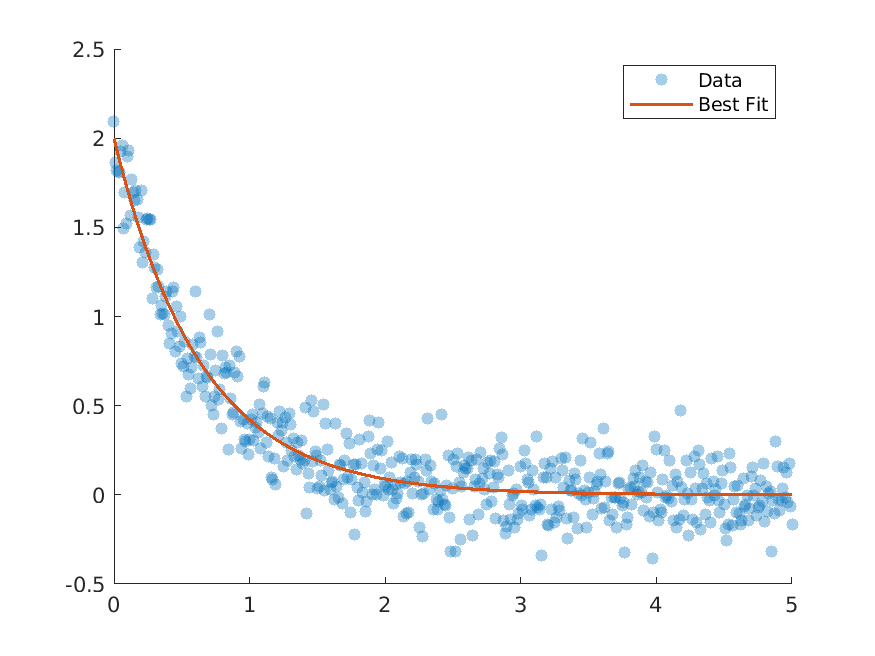
\includegraphics[width = \textwidth]{../figures/lsqcurvefit_performance.png}
  \caption{Performance of \texttt{lsqcurvefit}}
  \label{fig:lsqcurvefit_performance}
\end{figure}
\end{minipage}
\end{frame}
\end{document}